\documentclass[12pt]{article}
\usepackage[hidelinks]{hyperref}    
\usepackage[all]{hypcap}   
\usepackage{graphicx}
\usepackage{amsmath}
\usepackage{listings}
\usepackage{xcolor}
\usepackage{float}

% Define custom settings for HACK assembly language
\lstdefinelanguage
    [HACK]{Assembler}
    {morekeywords={@SP, @LCL, @ARG, @THIS, @THAT, @SCREEN, @KBD}, % Common HACK symbols
     alsoother={=,;,@},  % Symbols used in HACK assembly
     sensitive=true,     % Case-sensitive
     morecomment=[l]//,  % Define comments to start with "//"
    }

% Set up the listing style for HACK assembly
\lstset{
    language=[HACK]Assembler,
    basicstyle=\ttfamily\small,      % Small monospace font
    keywordstyle=\color{blue},       % Keywords in blue
    commentstyle=\color{gray},       % Comments in gray
    stringstyle=\color{red},         % Strings in red
    tabsize=4,
    showstringspaces=false,
    numbers=left,                    % Line numbers on the left
    numberstyle=\tiny\color{gray},
    breaklines=true,
    frame=single,                    % Frame around the code
}
\graphicspath{{../images/}}
\author{Andrea Malvezzi}
\title{\textbf{Architettura degli Elaboratori\\ Come implementare il computer HACK}}
\date{05 novembre, 2024}
\author{Andrea Malvezzi}
\begin{document}
\maketitle
\pagebreak
\tableofcontents
\pagebreak

\section{Premesse}
\label{sec:premises}
Il computer HACK sfrutta l'architettura Von Neumann a 16-bit, con una feature di quella Harvard:
la memoria dati viene separata da quella programma, in modo da poter caricare contemporaneamente dati e istruzioni.
\\
Questo viene reso possibile dal bus dati che, mentre nelle architetture moderne svolge due compiti distinti e quindi non eseguibili in parallelo, qui ne svolge solamente uno.
Conseguentemente per eseguire un'istruzione basta un ciclo di clock.

\section{La memoria}
\label{sec:memory}

\subsection{La ROM}
\label{ssec:ROM}
La ROM corrisponde ad un chip built-in che dato un address 15-bit codifica in binario
un'istruzione da eseguire, quindi: $\text{out} = \text{ROM}32\text{K}[address]$.

\subsection{Chip memory}
\label{ssec:memory_chip}
Il chip memory è composto da un totale di 3 componenti, per un totale di 24K indirizzi:
\begin{itemize}
    \item la RAM da 16K;
    \item il chip \textbf{Screen} da 8K, usato per mappare lo schermo;
    \item un singolo registro \textbf{Keyboard} per leggere il tasto premuto;
\end{itemize} 
Tuttavia, avendo in ingresso un address da 15 bit da convertire in binario, si sprecano molti indirizzi così facendo: $2^{15}=32767$ meno i 24576 occupati dal chip memory, per un totale di 8191 indirizzi sprecati. Cosa accade a questi?

\subsubsection{Il chip Screen}
\label{sssec:screen_chip}
All'interno del chip Screen si ha una corrispondenza diretta tra il singolo bit e un pixel sullo schermo. In base al valore di questi bit, lo schermo viene costsantemente refreshato colorando di bianco (0) o di nero (1) ogni singolo pixel.
\\
Per impostare il pixel in posizione (row, col) dello schermo ad un certo colore, occorrerà quindi settare il bit $col\%16$ della word all'indirizzo Screen[row*32 + col/16] a 1 oppure a 0.
\\
Ma come mai questi numeri? Anzitutto, occorre specificare che nel computer HACK lo schermo è composto da 256 righe e 512 colonne.
\\
Questo significa che in una singola riga ci saranno 512 caratteri, raggruppati in parole (che in informatica hanno spesso una grandezza di 16 bit),
da cui si evince che in una singola riga si avranno 32 parole ($512/16=32$). Ed ecco spiegato il \textbf{row*32}.
\\
Lo stesso ragionamento va applicato alle righe: avendo 256 righe, si avranno 16 ($256/16=16$) parole per colonna, da cui \textbf{col/16}.

\subsubsection{Esempio di codice per disegnare un rettangolo largo 16 pixel e alto MEM[0] pixel}
\label{sssec:rectangle_example}
\begin{lstlisting}
    @0              // A=0
    D=M             // D=RAM[0]

    @INFINITE_LOOP  // Preparo il salto
    D; JGE          // Se D>0

    @counter        // Variabile counter per iterare
    M=D             // RAM[counter]=RAM[0]

    @SCREEN         // Predefinita dal linguaggio
    D=A             // D=Indirizzo Screen
    @address        // Variabile address
    M=D             // RAM[address]=Indirizzo Screen

    (LOOP)
        @address    // Variabile address
        A=M         // A=Indirizzo Screen
        M=-1        // MEM[Indirizzo Screen]=-1
        
        @32         // A=32
        D=A         // D=32
        @address    // Variabile address
        M=M+D       // Address+=32

        @counter
        MD=M-1      // Counter--, D per check sul jump

        @LOOP       
        D;JGT       // Torno all'inizio

    (END)           // Ciclo dummy finale
        @END
        0;JMP
\end{lstlisting}

\subsubsection{Il chip Keyboard}
\label{sssec:keyboard_chip}
Come annunciato precedentemente questo chip è composto da un solo registro e fornisce in output la codifica ASCII estesa del tasto premuto, oppure 0 se non si preme alcun tasto.
\\
Il registro è read-only e vi sono alcuni tasti con codifiche particolari, come lo spazio.

\section{Comportamento della CPU}
\label{sec:CPU}
\begin{figure}[H]
    \centering
    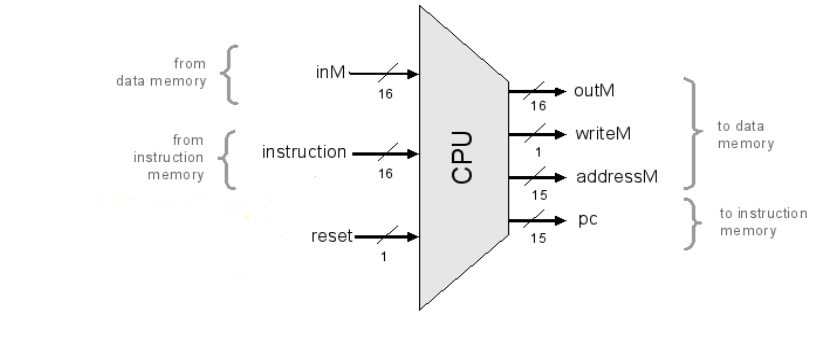
\includegraphics[width=1\textwidth, height=.7\textheight,keepaspectratio]{realizzare_HACK/CPU.png} % essenzialmente resiza l'immagine
    \begin{center}
        \caption{\label{fig:come_funziona_CPU}Schema logico CPU nell'architettura HACK.} % label fuori da caption spesso non va, mettilo dentro
    \end{center}
\end{figure}
La CPU è composta da 4 componenti: l'ALU e 3 registri, quali A, D, PC.
Questa esegue istruzioni seguendo le specifiche del linguaggio HACK (nel nostro caso). Ovvero:
\begin{itemize}
    \item i valori D ed A, se presenti, sono letti e/o scritti nei registri A ed M;
    \item il valore M, se presente nella right side dell'istruzione da eseguire, viene LETTO da inM (input-M);
    \item se invece il valore M risulta presente nella left side dell'istruzione da eseguire, allora
            l'output verrà scritto in outM, A prenderà il valore di addressM e writeM verrà alzato ad 1.
\end{itemize}

% TODO: slide 16 continua

\section{Codifica A-Instruction}


\end{document}